\section{Moravec}\label{sec:moravec}
Moravec's hjørne detektor, beskrevet i \cite{moravec}, er en af de tidligste feature detektorer, og definere et hjørne som værende et område, hvor der opstår store intensitetsskift. Moravec anvender denne definition til at opnå en matematisk formulering af hjørner ved at bygge videre på notationen om et kvadratisk vindue, omliggende det undersøgte punkt, diskuteret i \ref{subsec:corner}, typisk i størrelser af 3x3, 5x5 eller 7x7 pixel regioner. De interessante punkter findes når auto-korrelationen imellem de forskudte billeder er stor. Forskydningsvinduet kan derved bruges til at detektere hjørner, ved at tage et pixel område omkring et punkt, forskyde dette vindue med én pixel i alle principielle retninger (horisontalt, vertikalt og diagonalt) og udregne intensitetsvariationen. Denne variation kan beskrives med en vægtet funktion over vinduet  \emph{(MSSD: Mean Summed Square Difference)}, der udregner forskellen på vinduerne:
\begin{equation}
E(u,v)= \sum w(x,y)[I(x,y)-I(x+u,y+v)]^2     
\end{equation}
hvor $(u,v)\in \lbrace -1,0,1 \rbrace$ er forskydningsvektoren, der summere over alle pixels i vinduet. Den mindste forskel i de otte skift, definere punktets \textit{hjørnestyrke}.
$$
C(x,y)=min(E(u,v))
$$
Den mindste forskel tages da et punkt, der er lokaliseret langs en kant, resultere i et stort intensitetsskifte når kanten krydses, men lille skift ved bevægelse langs kanten, hvor hjørner opstår når intensitetsvariationen er stor i alle retninger. Der opstilles en grænseværdi for $C$, der bestemmer, hvornår der opstår et hjørne. Figur \ref{fig:moravec} illustrere en udregning af \textit{MSSD} af et diagonalt skift på en isoleret sort pixel (med en intensitet på 0) på en hvid baggrund (med en intensitet på 255) og på et idealt hjørne. Det røde vindue indikere det originale vindue og det blå indikere  vinduet forskudt med vektoren $u = (1,1)$. 
\begin{figure}[H]
    \centering
    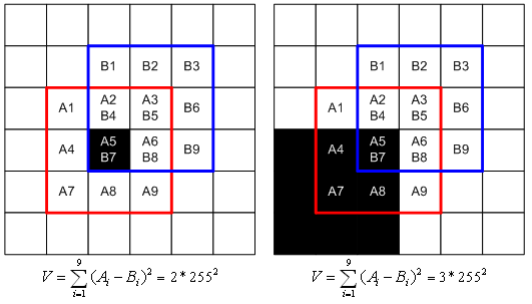
\includegraphics[width=0.45\textwidth]{fig/25.png}
     \vspace{-1em}
    \begin{center}    
       \caption{\textcolor{gray}{\footnotesize \textit{ WSSD udregninger for intensitetsvariationer imellem forskudte vindue. }}}
    \label{fig:moravec}
     \end{center}
     \vspace{-2.5em}
  \end{figure} \noindent
Moravec lider af følgende problemer pga. dens simplicitet. 
\begin{itemize}
\item{ Der undersøges kun et diskret sæt af pixelskift (i hver principiel orientering) og resultatet er derfor anisotropisk\footnote{Afhængig af retning}. Undersøges en kant, der ikke er horisontal, vertikal eller diagonal ift. punktet vil den mindste intensitetsvariation være stor, og derved kan punktet fejlagtigt detekteres som et hjørne.}
\item{Det skiftende vindue er rektangulær og binært, metoden er derfor meget følsom overfor støj i billedet.}
\item{Detektoren finder punkter lokaliseret på kanter. I sektion \ref{subsec:kant} defineres en kant som værende et pludseligt skift i intensiteten i en given retning. Små deformationer i kanterne som støj, vil resultere i at den mindste intensitetsvariation vil være relativt stor, og derfor detektere punktet som værende et interessepunkt.}
\end{itemize}
% <evt konklusion>
% <måske billeder download cornerdetection.pdf>
\subsection*{Algoritme:}
\begin{enumerate}
\item{For hvert pixel i billedet, udregnes auto-korrelationen imellem skift af $(u,v) \in [-1,0,1]$. udregnet ved \textit{MSSD} }
\item{\textit{"Hjørnestyrken"} udregnes for hvert pixel ved at finde $C(x,y)=min(E(u,v))$ }
\item{ En grænseværdi sættes sættes for $C(x,y)$}
\item{lokale ekstremaer identificeres. }
\end{enumerate}
\subsection*{Konklusion}
Moravec er som nævnt en simpel algoritme, med mange udfordringer, der gør at den ikke bruges som en repeterbar detektor. Detektoren er i dag ikke i sig selv relevant, som den var da den blev udgivet, men bygges videre på i andre detektorer, f.eks. \cite{Harris} beskrevet i sektion, \ref{sec:harris} som direkte tilgår de nævne problemstillinger med Moravec.